
\documentclass[iicol]{sn-jnl}

\usepackage{graphicx}%
\usepackage{multirow}%
\usepackage{amsmath,amssymb,amsfonts}%
\usepackage{amsthm}%
\usepackage{mathrsfs}%
\usepackage[title]{appendix}%
\usepackage{xcolor}%
\usepackage{textcomp}%
\usepackage{siunitx}%
\usepackage{manyfoot}%
\usepackage{booktabs}%
\usepackage{algorithm}%
\usepackage{algorithmicx}%
\usepackage{algpseudocode}%
\usepackage{listings}%
\usepackage{adjustbox}%
\usepackage{tabularx}
\usepackage{tikz}
\usepackage{pgfplots}
\pgfplotsset{compat=1.17}
\usepackage[numbers]{natbib}
\usepackage{enumitem}

\raggedbottom

\begin{document}

\title{Scale-Invariant State Representation and Maximum-Entropy Deep Reinforcement
       Learning for Task Offloading in Vehicular Edge Computing}

\author*[1,2]{\fnm{Antônio Sérgio de Sousa} \sur{Vieira}}
              \email{sergio.vieira@ifce.edu.br}
\author[1,3]{\fnm{Alisson Barbosa de} \sur{Souza}}
             \email{alisson@ufc.br}
\author[1]{\fnm{Joaquim} \sur{Celestino Júnior}}
           \email{joaquim.celestino@uece.br}

\affil*[1]{\orgdiv{Intelligent Networks and Systems Group (INETSYS)},
           \orgname{State University of Ceará},
           \orgaddress{\city{Fortaleza}, \country{Brazil}}}
\affil[2]{\orgname{Federal Institute of Education, Science and Technology},
          \orgaddress{\city{Itapipoca}, \country{Brazil}}}
\affil[3]{\orgname{Federal University of Ceará},
          \orgaddress{\city{Quixadá}, \country{Brazil}}}

\abstract{%
Task offloading in Vehicular Edge Computing (VEC) networks is a critical mechanism to satisfy the stringent latency and energy constraints of advanced
autonomous applications. The high mobility of vehicles creates an environment in which the number of
available edge servers and neighboring vehicles changes continuously, so the observation space is \emph{dimensionally variable}.
This variability prevents standard Deep Reinforcement Learning (DRL) agents
from generalizing across vehicular densities without costly retraining.
To address this challenge, this paper proposes \textbf{SAC-FTOPSIS}, a hybrid
decision-making architecture that integrates the Technique for Order of
Preference by Similarity to Ideal Solution (TOPSIS) with the Soft Actor-Critic
(SAC) algorithm.
The TOPSIS module evaluates every candidate offloading node—each characterized
by Job Completion Time (JCT), energy consumption, and physical distance—using
$L_1$-Manhattan distances and weights $[0.4, 0.3, 0.3]$, and then compresses
the variable-size observation into a \emph{fixed} 6-dimensional, scale-invariant
state vector.
A SAC agent receives this compact representation and learns a binary policy:
execute locally or offload to the top-ranked candidate.
Entropy regularization prevents the policy from collapsing into deterministic
local-only or offload-only modes.
Extensive simulation across 601 heterogeneous Vehicle-to-Everything (V2X) and
5G scenarios demonstrates that the TOPSIS integration consistently improves
every tested DRL family: SAC improves from $4.47\%$ to $44.36\%$
($+39.9$\,pp), TD3 from $41.62\%$ to $43.01\%$ ($+1.4$\,pp), and PPO from
$41.61\%$ to $41.95\%$ ($+0.3$\,pp) in deadline compliance rate.
Among all evaluated policies, SAC-FTOPSIS achieves the highest compliance
($44.36\%$) and the highest Success-Weighted Quality (SWQ) index ($0.1450$).
Crucially, the model is trained on a single density regime and generalizes
\emph{zero-shot} to unseen vehicular densities ranging from 10 to
\SI{30}{tasks\per\second}.%
}

\keywords{Task offloading, Vehicular Edge Computing, Soft Actor-Critic,
          TOPSIS, Multi-criteria state compression, Zero-shot generalization}

\maketitle

%─────────────────────────────────────────────────────────────────────────────
\section{Introduction}
\label{sec:intro}
%─────────────────────────────────────────────────────────────────────────────

\paragraph{Context and motivation.}
The steady cost reduction of semiconductor and communication technologies
has enabled a new generation of intelligent vehicle applications demanding
simultaneously high efficiency, usefulness, reliability, and
safety~\cite{uddin2024intelligent}.
Advanced driver assistance systems, real-time object detection, cooperative
perception, and V2X path planning impose latency budgets often below
\SI{10}{\milli\second}~\cite{3gppRel17}, requiring enormous on-demand
computation at the network edge.
Fifth-generation New Radio (5G~NR) and its successor 6G provide unprecedented
communication throughput and ultra-low radio latency, effectively eliminating
the transmission bottleneck for short payloads.
However, lower propagation latency does not eliminate the
\emph{processing} challenge: modern vehicular applications generate massive
volumes of sensor data—LiDAR point clouds, HD maps, multi-camera streams—whose
end-to-end response time and energy cost remain critical
constraints~\cite{zhou2019,zhang2018}.

\paragraph{MEC and VEC as solutions.}
Mobile Edge Computing (MEC) and its vehicular specialization, Vehicular Edge
Computing (VEC), address these constraints by co-locating compute resources with
the radio access network~\cite{mao2017}.
Vehicles can offload computation-intensive tasks to Road-Side Unit (RSU) servers
via 5G~C-V2X or to neighboring vehicles via direct V2V sidelink, dramatically
reducing both response time and onboard energy
consumption~\cite{huang2020,fang2021mec_iot}.

\paragraph{Heterogeneous OBU capacity and cooperative computing.}
A key observation in modern vehicular environments is that On-Board Units
(OBUs) are \emph{heterogeneous}: high-end vehicles equipped with powerful
processing units (GPUs, NPUs) may temporarily carry underutilized capacity,
while compact vehicles operate near their computational limits.
This heterogeneity creates cooperative computing opportunities in which
resource-rich neighbors can absorb tasks from resource-constrained
ones, improving Quality of Service (QoS) for the entire
Intelligent Transportation System (ITS)~\cite{he2019d2d_mec_twc}.
Realizing this potential, however, requires offloading policies that are aware
of the network's shifting topology and can reason about multi-hop, multi-criteria
trade-offs in real time.

\paragraph{Challenges and research gaps.}
Despite a growing body of literature, several critical gaps remain open, as
systematically identified by Miriyala and
Chirra~\cite{miriyala2026dl_offload_review}.
Most evaluation studies rely on simplified, static scenarios—fixed number of
vehicles, uniform task distributions, idealized channel models—that fail to
capture the high dynamism of real vehicular networks.
Consequently, policies that perform well in synthetic benchmarks often degrade
sharply when vehicular density or traffic regime changes.

\paragraph{Why classical strategies fall short.}
Task offloading is fundamentally a multi-criteria optimization problem.
\emph{Heuristics} such as greedy strategies have been widely deployed due to
their simplicity~\cite{ahmed2022survey}, but they evaluate only the current
network snapshot and are unable to anticipate queue saturation or
future task arrivals.
\emph{Metaheuristics} (genetic algorithms, particle swarm optimization, ant
colony optimization) offer stronger global search guarantees and have been
applied to static offloading~\cite{li2020genetic,you2021efficient,kishor2022task},
yet they are fundamentally ill-suited to vehicular environments: their
population-based search requires tens to hundreds of fitness evaluations per
decision instant, which is incompatible with sub-second deadlines; they must
be rerun from scratch every time the topology changes; and their initialization
becomes increasingly non-trivial as the network grows.

\paragraph{Deep Reinforcement Learning and its limitations.}
Deep Reinforcement Learning (DRL) is a natural fit for task offloading because
it learns a \emph{policy}—a mapping from observations to actions—that implicitly
accounts for future consequences, not just the current state~\cite{huang2020,shi2023}.
Unlike heuristics and metaheuristics, a DRL agent can exploit temporal
correlations in traffic patterns and queue dynamics learned from experience.
Nevertheless, standard DRL architectures share a critical weakness: they
require \emph{retraining} whenever the operational scenario
changes~\cite{miriyala2026dl_offload_review}.
Because the neural network input is a fixed-size vector, any change in the
number of candidate offloading nodes—caused by vehicles entering or leaving
communication range—invalidates the trained model.
Zero-padding absent candidates is a common workaround but introduces spurious
inputs that destabilize learning and reduce the policy's ability to generalize.

\paragraph{Our prior work and the path to SAC-FTOPSIS.}
In our previous work, we proposed FOFF~\cite{vieira2025foff}, a
Fuzzy-TOPSIS framework that ranks edge servers in a \emph{static} VEC scenario
using linguistic criteria weights to handle uncertainty.
FOFF demonstrated that multi-criteria methods can achieve strong energy
efficiency and QoS without any training phase.
Its limitation is precisely the lack of adaptation: Fuzzy-TOPSIS selects the
best candidate by a fixed scoring rule and cannot improve from experience or
adjust to non-stationary traffic.
Building on these insights, we now propose \textbf{SAC-FTOPSIS}: a hybrid
architecture that delegates the multi-criteria \emph{candidate evaluation}
to TOPSIS while delegating the long-horizon \emph{policy optimization} to the
Soft Actor-Critic (SAC) algorithm, combining the local optimality of MCDM with
the forward-looking capability of DRL.

\paragraph{Contributions.}
The main contributions of this paper are:
\begin{enumerate}[leftmargin=*,nosep]
  \item \textbf{Challenging, realistic evaluation scenario.}
        We evaluate all policies on 601~heterogeneous VEC scenarios spanning
        five vehicular density regimes ($10$–$\SI{30}{tasks\per\second}$), with
        realistic 5G and V2V channel models, heterogeneous OBU frequencies,
        and per-task deadlines drawn from a continuous distribution.

  \item \textbf{Scale-invariant state representation.}
        TOPSIS compresses the variable-size candidate set into a fixed 6D
        vector whose components are normalized ratios and relative differences,
        making it valid regardless of the number of available candidates.
        This representation enables \emph{zero-shot generalization}: a model
        trained on one density regime transfers directly to unseen regimes
        without retraining.

  \item \textbf{Low-complexity decision architecture.}
        By reducing the action space to a single bit (local vs.\ rank-1
        offload), the agent avoids exponential action-space growth and runs
        inference in $O(1)$ neural-network forward passes per task—suitable
        for onboard real-time deployment.

  \item \textbf{Principled reward shaping.}
        The deadline-aware reward function provides a continuous gradient
        signal in both the success and failure regimes, preventing reward
        sparsity and teaching the agent to minimize tardiness rather than
        merely avoid it.

  \item \textbf{Complementary decision horizons.}
        TOPSIS provides the best \emph{local} solution given current network
        conditions; SAC learns the best \emph{long-term} policy by looking
        ahead through accumulated experience.
        The combination yields results that neither component can achieve alone.
\end{enumerate}

Evaluated across 601~scenarios, SAC-FTOPSIS achieves a deadline compliance rate
of $44.36\%$ and SWQ of $0.1450$—the best among all DRL and heuristic
baselines—while the raw-state SAC-Base achieves only $4.47\%$ under the same
training budget.

The remainder of the paper is structured as follows.
Section~\ref{sec:related} reviews related work.
Section~\ref{sec:model} formalizes the system model and optimization objective.
Section~\ref{sec:arch} describes the SAC-FTOPSIS architecture in detail.
Section~\ref{sec:eval} presents the experimental evaluation.
Section~\ref{sec:conclusion} concludes the paper.

%─────────────────────────────────────────────────────────────────────────────
\section{Related Work}
\label{sec:related}
%─────────────────────────────────────────────────────────────────────────────

\subsection{Task Offloading in VEC}

Task offloading optimization has been extensively studied as a mixed latency-
energy trade-off~\cite{liu2022multitask_mec,fang2021mec_iot}.
Early works relied on deterministic multi-criteria decision-making (MCDM)
methods.
The FOFF framework~\cite{vieira2025foff} applied Fuzzy-TOPSIS to rank edge
servers by latency and energy without any training phase, achieving significant
energy savings.
However, purely rule-based methods cannot adapt to non-stationary queuing
dynamics or learn from historical performance.
Hybrid approaches that combine MCDM pre-filtering with a learned policy are an
active research direction~\cite{uddin2024intelligent}.

\subsection{Deep Reinforcement Learning for VEC}

DRL-based offloading has gained traction for its ability to adapt online.
Deep Q-Networks (DQN) and their dueling variants address the discrete-action
case~\cite{3459991.pdf}, while actor-critic algorithms (PPO, DDPG, TD3)
handle continuous or high-dimensional settings~\cite{schulman2017ppo}.
A common limitation is the fixed-input-size assumption: most models use
zero-padding to accommodate up to a maximum number of candidates, introducing
spurious symmetry-breaking artifacts and reducing generalization.
Off-policy algorithms (SAC, TD3) offer better sample efficiency than on-policy
methods, but are still susceptible to representation collapse when the state is
uninformative~\cite{haarnoja2018sac}.

\subsection{Positioning of SAC-FTOPSIS}

Prior work has combined MCDM methods with DRL for MEC, but these typically
treat MCDM as a post-processing filter (ranking the DRL action set) rather than
as a \emph{state-engineering} step.
SAC-FTOPSIS is, to our knowledge, the first architecture to use TOPSIS
\emph{inside the observation pipeline}: its output is not a decision but a
compact, scale-invariant state encoding that enables DRL training without
zero-padding or fixed topology assumptions.
Crucially, this state compression is \emph{algorithm-agnostic}: our experiments
show that pairing the TOPSIS state with SAC, TD3, and PPO each yields
consistent improvements over their respective raw-state baselines, confirming
that the representation itself—rather than any particular DRL algorithm—is the
primary driver of generalization.

%─────────────────────────────────────────────────────────────────────────────
\section{System Model and Problem Formulation}
\label{sec:model}
%─────────────────────────────────────────────────────────────────────────────

\subsection{Network Model}

We consider a heterogeneous VEC environment with one client vehicle $v_0$, one
RSU server accessible via 5G C-V2X (uplink bandwidth $B_{\mathrm{V2I}}$), and
a time-varying set $\mathcal{V}(t)$ of neighboring vehicles accessible via V2V
sidelink (bandwidth $B_{\mathrm{V2V}}$).
The RSU has a service queue of capacity $Q_{\mathrm{RSU}}$; each vehicle
$v \in \mathcal{V}(t)$ has a local queue $Q_v$.

\subsection{Task Model}

Each task $\tau_j = (C_j, D_j, s_j)$ is characterized by its CPU complexity
$C_j$ (cycles), deadline $D_j$ (seconds), and input data size $s_j$ (bits).
Three execution \emph{modes} are available:
\begin{itemize}[nosep,leftmargin=*]
  \item \textbf{Local ($m=0$):} executed on $v_0$ with frequency $f_{\mathrm{loc}}$.
  \item \textbf{RSU ($m=1$):} uploaded to the RSU and executed at $f_{\mathrm{RSU}}$.
  \item \textbf{V2V ($m=2$):} offloaded to a neighboring vehicle $v^* \in \mathcal{V}(t)$.
\end{itemize}
A mode $m$ is \emph{feasible} if the corresponding peer is within communication
range and its queue is not full.

\subsection{Latency Model}

The Job Completion Time of mode $m$ for task $\tau_j$ is
\begin{equation}
  \mathrm{JCT}_j^{(m)} = t_j^{\mathrm{tx},(m)} + t_j^{\mathrm{queue},(m)}
                         + \frac{C_j}{f^{(m)}},
  \label{eq:jct}
\end{equation}
where $t_j^{\mathrm{tx},(m)}$ is the transmission time (upload), and
$t_j^{\mathrm{queue},(m)}$ is the residual waiting time in the target queue,
estimated as the remaining execution time of tasks already in the queue.

\subsection{Energy Model}

The energy consumed for mode $m$ is
\begin{equation}
  E_j^{(m)} = \alpha_c^{(m)} \bigl[V^{(m)}\bigr]^2 C_j
             + P_{\mathrm{TX}}^{(m)}\,t_j^{\mathrm{tx},(m)},
  \label{eq:energy}
\end{equation}
where $\alpha_c^{(m)}$ is the chip capacitance, $V^{(m)}$ is the supply voltage
at frequency $f^{(m)}$, and $P_{\mathrm{TX}}^{(m)}$ is the transmit power.
For the local mode, the transmit term is zero.

\subsection{Optimization Objective}

The per-task QoS contribution is
\begin{equation}
  \Phi_j = \alpha\,\mathrm{JCT}_j + \beta\,E_j
            + \gamma\,\mathbf{1}[\mathrm{JCT}_j > D_j]\,\mathrm{JCT}_j,
  \label{eq:obj}
\end{equation}
with $\alpha=\beta=0.5$ and a deadline-miss penalty coefficient $\gamma=0.015$.
The system objective is to minimize $\sum_j \Phi_j$ while maximizing the
\emph{deadline compliance rate} $\hat{\tau} = |\{j : \mathrm{JCT}_j \le D_j\}|/N$.

%─────────────────────────────────────────────────────────────────────────────
\section{The SAC-FTOPSIS Architecture}
\label{sec:arch}
%─────────────────────────────────────────────────────────────────────────────

Figure~\ref{fig:architecture} depicts the complete architecture.
At each decision instant, the TOPSIS module processes the multi-criteria
information about all feasible candidates and produces the 6D state vector
that is passed to the SAC agent.

\begin{figure}[t]
  \centering
  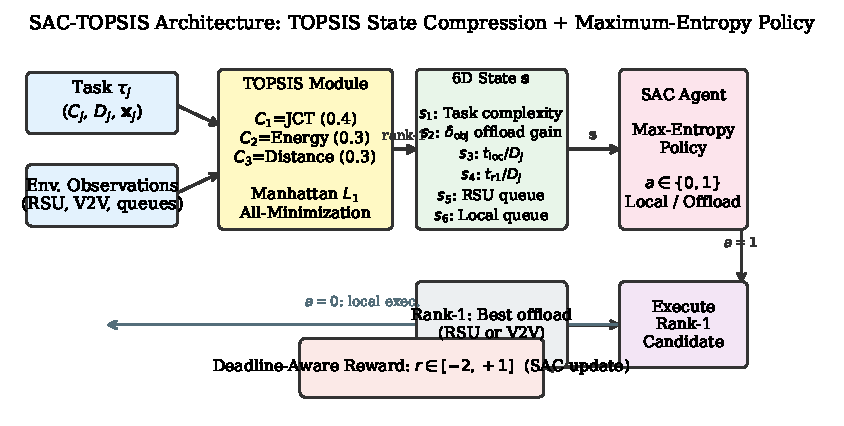
\includegraphics[width=\columnwidth]{images/fig_01_architecture.pdf}
  \caption{SAC-FTOPSIS architecture.
           TOPSIS compresses the variable-size candidate set into a fixed 6D
           scale-invariant state vector.
           SAC learns a binary policy (local vs.\ rank-1 offload) on this
           representation with maximum-entropy regularization.}
  \label{fig:architecture}
\end{figure}

\subsection{TOPSIS-Based State Compression}
\label{sec:topsis}

\paragraph{Decision matrix.}
For task $\tau_j$, we build a $3 \times 3$ decision matrix
$\mathbf{X} \in \mathbb{R}_{\ge 0}^{3\times 3}$ whose rows correspond to the
three candidate modes (local, RSU, V2V) and whose columns are the three
\emph{cost} criteria:
\begin{equation}
  \mathbf{X} =
  \begin{bmatrix}
    \mathrm{JCT}_j^{(0)} & E_j^{(0)} & 0 \\
    \mathrm{JCT}_j^{(1)} & E_j^{(1)} & d_{\mathrm{RSU}} \\
    \mathrm{JCT}_j^{(2)} & E_j^{(2)} & d_{\mathrm{V2V}}
  \end{bmatrix},
  \label{eq:dm}
\end{equation}
where $d_{\mathrm{RSU}}$ and $d_{\mathrm{V2V}}$ are the Euclidean distances
to the RSU and the selected V2V peer, respectively.
If a mode is infeasible its row is set to $10^6$ to exclude it from the ideal
solutions.

\paragraph{Weighted normalization.}
Each column $j$ is normalized by its Euclidean norm $\|\mathbf{X}_{:j}\|_2$,
then multiplied by weight $w_j \in \{0.4, 0.3, 0.3\}$ (JCT, energy,
distance), yielding the weighted normalized matrix $\widetilde{\mathbf{X}}$.

\paragraph{$L_1$-Manhattan TOPSIS.}
We depart from classic TOPSIS by measuring distances to the positive ideal
solution (PIS) $A^+$ and negative ideal solution (NIS) $A^-$ using the
\emph{Manhattan} ($L_1$) norm:
\begin{equation}
  D_i^+ = \textstyle\sum_{k} \lvert \widetilde{x}_{ik} - A_k^+ \rvert,
  \qquad
  D_i^- = \textstyle\sum_{k} \lvert \widetilde{x}_{ik} - A_k^- \rvert.
  \label{eq:manhattan}
\end{equation}
The proximity score is then $\mathcal{C}_i = D_i^- / (D_i^+ + D_i^-)$.
Because all criteria are cost-minimization objectives, $A^+$ is the
column-wise minimum and $A^-$ is the column-wise maximum of
$\widetilde{\mathbf{X}}$.
The $L_1$ metric is less sensitive to outliers—a critical property when
queue estimates are noisy—and computationally lighter than $L_2$.

\paragraph{Rank-1 selection.}
The rank-1 offload candidate is the feasible \emph{non-local} mode with the
highest $\mathcal{C}_i$:
\begin{equation}
  m^* = \operatorname*{argmax}_{i \in \{1,2\}} \mathcal{C}_i
        \;\text{s.t.\ mode } i \text{ is feasible}.
  \label{eq:rank1}
\end{equation}
Ties are broken in favour of V2V to encourage load balancing.
If no offload mode is feasible, $m^*$ defaults to local execution regardless
of the agent's action.

\paragraph{6D state vector.}
The state $\mathbf{s} \in \mathbb{R}^6$ is assembled as:
\begin{align}
  s_1 &= C_j / 10^{10}                          & &\text{(task complexity, normalized)} \notag\\
  s_2 &= \mathrm{clip}\!\left(1 - \frac{\mathrm{cost}_{m^*}}
                                              {\mathrm{cost}_{\mathrm{loc}}},\,-1,1\right)
         & &\text{(objective-level offload advantage)} \notag\\
  s_3 &= \min\!\left(1,\; \mathrm{JCT}^{(0)} / D_j\right)
         & &\text{(local urgency ratio)} \notag\\
  s_4 &= \min\!\left(1,\; \mathrm{JCT}^{(m^*)} / D_j\right)
         & &\text{(rank-1 urgency ratio)} \notag\\
  s_5 &= \min\!\left(1,\; |Q_{\mathrm{RSU}}| / 25\right)
         & &\text{(RSU queue occupancy)} \notag\\
  s_6 &= \min\!\left(1,\; |Q_{v_0}| / 25\right)
         & &\text{(local vehicle queue occupancy),}
  \label{eq:state}
\end{align}
where $\mathrm{cost}_m = \alpha\,\mathrm{JCT}^{(m)} + \beta\,E^{(m)}$.
All components lie in $[0,1]$ or $[-1,1]$, making $\mathbf{s}$
\emph{scale-invariant}: it does not depend on the number of available
candidates, only on the relative quality of the best one.

\subsection{Maximum-Entropy Soft Actor-Critic}
\label{sec:sac}

The SAC agent optimizes the maximum-entropy objective~\cite{haarnoja2018sac}:
\begin{equation}
  \pi^* = \operatorname*{argmax}_\pi\;
  \mathbb{E}_{\tau \sim \pi}\!\left[
    \sum_{t} \gamma^t \bigl(r_t + \alpha_T\,\mathcal{H}[\pi(\cdot\mid s_t)]\bigr)
  \right],
  \label{eq:sac_obj}
\end{equation}
where $\alpha_T$ is the automatically tuned temperature parameter.
The actor and critic networks are MLPs with two hidden layers of 256~units and
ReLU activations.
The actor outputs logits for the Bernoulli action distribution; the
temperature $\alpha_T$ is adapted to a target entropy of $\log 2 / 2$ nats.
The replay buffer holds $10^5$ transitions; mini-batch size is $256$; the
learning rate is $3 \times 10^{-4}$ for all networks.

\paragraph{Why binary action?}
Delegating the \emph{selection} of the offload destination to TOPSIS reduces
the action space from $|\mathcal{V}(t)| + 2$ dimensions to a single bit.
This simplification is lossless from the agent's perspective because the
relative ordering of candidates is already encoded in $s_2$--$s_4$.

\subsection{Deadline-Aware Reward Function}
\label{sec:reward}

The reward $r_j$ for task $\tau_j$ is designed to guide the agent toward
deadline compliance while providing a continuous gradient signal:
\begin{equation}
  r_j = \begin{cases}
    1.0 - 0.5 \cdot \rho_j        & \text{if } \mathrm{JCT}_j \le D_j, \\
    -1.0 - \min(1,\,\delta_j)     & \text{otherwise,}
  \end{cases}
  \label{eq:reward}
\end{equation}
where
\begin{equation}
  \rho_j = \tfrac{1}{2}\!\left(\frac{\mathrm{JCT}_j}{D_j}
                              + \frac{E_j}{E_{\max,j}}\right) \in [0,1]
  \label{eq:rho}
\end{equation}
is a normalized cost ratio, and $\delta_j = (\mathrm{JCT}_j - D_j)/D_j$ is
the relative deadline overrun.
Successful executions yield $r_j \in [0.5,\,1.0]$: faster, more efficient
tasks receive higher rewards.
Failed executions yield $r_j \in [-2,\,-1]$: the penalty grows with the degree
of tardiness, providing a gradient that teaches the agent to \emph{fail
by the least amount possible}.

%─────────────────────────────────────────────────────────────────────────────
\section{Performance Evaluation}
\label{sec:eval}
%─────────────────────────────────────────────────────────────────────────────

\subsection{Simulation Setup}

All algorithms run on a custom discrete-event VEC simulator written in C++20
with \texttt{simcpp20} and the Armadillo linear-algebra library.
Neural networks are trained and exported using LibTorch (PyTorch C++ API).
Mobility scenarios are generated with realistic V2X parameters: vehicular
speeds of \SI{30}{\kilo\meter\per\hour} to \SI{120}{\kilo\meter\per\hour},
5G uplink bandwidth \SI{20}{\mega\hertz}, V2V sidelink \SI{10}{\mega\hertz},
RSU frequency $f_{\mathrm{RSU}} = \SI{2}{\giga\hertz}$, and onboard
$f_{\mathrm{loc}} \in [0.5, 1.0]$\,GHz.
Task deadlines follow a truncated Gaussian over $[0.05, 2.0]$\,s;
CPU complexity $C_j \sim \mathrm{Uniform}[10^8, 10^{10}]$ cycles.

\paragraph{Training.}
All DRL agents are trained for 400 episodes on scenarios with a fixed
vehicular density of \SI{10}{tasks\per\second}.
Each training episode simulates 100 task arrivals with a new mobility
realization drawn from the same distribution.

\paragraph{Test.}
After training, agents are evaluated \emph{zero-shot} across 601 test
scenarios covering five density regimes:
$\{10, 15, 20, 25, 30\}$~tasks/s.
No further learning or adaptation occurs during testing.

\paragraph{Baselines.}
We compare against:
\emph{Always-Local} (never offloads),
\emph{Greedy} (always offloads to the V2V peer with the shortest estimated
JCT, an optimistic oracle baseline),
\emph{Greedy-Fair} (greedy with Jain fairness constraint),
\emph{Random} (offloads to a randomly selected peer),
\emph{SAC-Base} (SAC with a raw 11-dimensional state vector, no TOPSIS),
\emph{PPO-TOPSIS} (on-policy PPO with the same 6D TOPSIS state),
and \emph{TD3-TOPSIS} (off-policy TD3 with the same 6D TOPSIS state).

\paragraph{Metrics.}
\begin{itemize}[nosep,leftmargin=*]
  \item \textbf{Deadline compliance rate}: fraction of tasks with
        $\mathrm{JCT}_j \le D_j$.
  \item \textbf{Success-Weighted Quality (SWQ)}:
        $\mathrm{SWQ} = \hat{\tau} \cdot
         \overline{\bigl[(D_j - \mathrm{JCT}_j)/D_j\bigr]}_{\mathrm{success}}$,
        which rewards meeting deadlines with large slack.
  \item \textbf{Mean JCT} and \textbf{total energy consumed}.
\end{itemize}

\subsection{Overall Performance Comparison}

Figure~\ref{fig:performance} and Table~\ref{tab:results} summarize
the aggregate performance over all 601 test scenarios.

\begin{figure}[t]
  \centering
  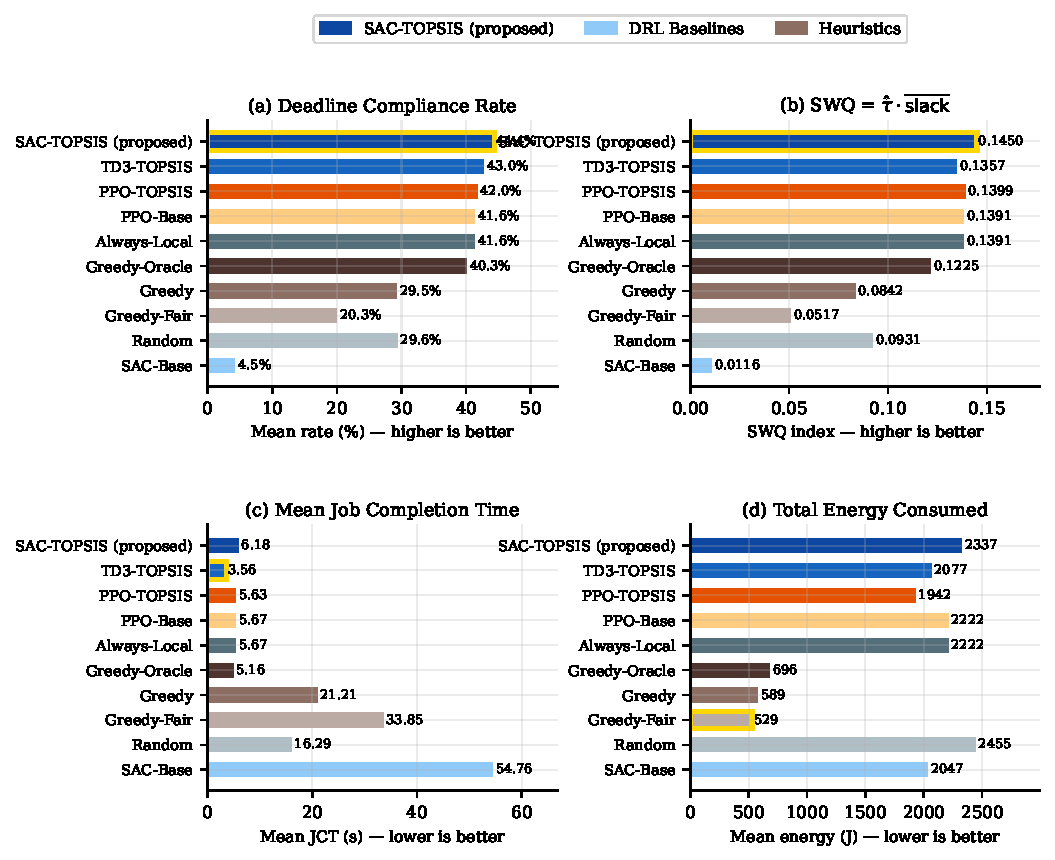
\includegraphics[width=\columnwidth]{images/fig_02_performance.pdf}
  \caption{Performance comparison across key metrics.
           SAC-FTOPSIS (dark blue) achieves the highest deadline compliance rate
           and SWQ index.
           The gold border marks the best value in each chart.}
  \label{fig:performance}
\end{figure}

\begin{table}[t]
\caption{Aggregate performance over 601 test scenarios
         (mean over scenarios, densities $\{10,15,20,25,30\}$~tasks/s).
         Arrows ($\uparrow$) show the gain from adding TOPSIS to each base
         algorithm. Bold denotes the best DRL value; $\dagger$ marks the
         oracle baseline.}
\label{tab:results}
{\small
\begin{tabular}{lrrrr}
\toprule
\textbf{Policy} & \textbf{Deadline (\%)} & \textbf{SWQ} &
\textbf{JCT (s)} & \textbf{Energy (J)} \\
\midrule
SAC-Base               &  4.47 & 0.0116 & 54.76 & 2047 \\
SAC-FTOPSIS (ours) $\uparrow\mathbf{+39.9}$ & \textbf{44.36} & \textbf{0.1450} & 6.18 & 2337 \\
\midrule
TD3-Base               & 41.62 & 0.1391 &  \textbf{3.53} & 2222 \\
TD3-TOPSIS $\uparrow+1.4$  & 43.01 & 0.1357 &  3.56 & 2077 \\
\midrule
PPO-Base               & 41.61 & 0.1391 &  5.67 & 2222 \\
PPO-TOPSIS $\uparrow+0.3$  & 41.95 & 0.1399 &  5.63 & \textbf{1942} \\
\midrule
Always-Local           & 41.61 & 0.1391 &  5.67 & 2222 \\
\midrule
Greedy-Oracle$^\dagger$ & 40.31 & 0.1225 &  5.16 &  696 \\
Greedy                 & 29.54 & 0.0842 & 21.21 &  589 \\
Greedy-Fair            & 20.26 & 0.0517 & 33.85 &  529 \\
Random                 & 29.61 & 0.0931 & 16.29 & 2455 \\
\bottomrule
\end{tabular}}
\end{table}

\paragraph{TOPSIS consistently improves every DRL family.}
Table~\ref{tab:results} reveals a result that is central to this paper:
pairing TOPSIS with any tested DRL algorithm improves deadline compliance
over the corresponding base version.
The magnitude of the gain, however, varies substantially across algorithm
families and reflects the interaction between the TOPSIS state and each
algorithm's exploration strategy.

\emph{SAC} experiences the most dramatic improvement:
SAC-Base achieves only $4.47\%$ compliance because it converges to an
almost-always-offload policy ($94.9\%$ V2V), incurring prohibitive queueing
delays whenever neighbors are congested.
Adding the TOPSIS state rescues the policy to $44.36\%$ ($\mathbf{+39.9}$\,pp),
the best result across all evaluated policies.
The 6D representation provides the semantic signal—urgency ratios and
queue occupancies—that SAC needs to distinguish beneficial from harmful offload
decisions.

\emph{TD3} already collapses to always-local in its base form ($41.62\%$,
identical to Always-Local), because its deterministic policy avoids the risky
V2V path without exploration pressure.
With the TOPSIS state, TD3 learns to exploit V2V opportunistically
($23.4\%$), raising compliance to $43.01\%$ ($+1.4$\,pp) and achieving
the lowest mean JCT ($3.56$\,s) of any policy.

\emph{PPO} also collapses to always-local in its base form ($41.61\%$) due
to high on-policy gradient variance.
The TOPSIS state provides marginal improvement to $41.95\%$ ($+0.3$\,pp).
The gain is limited because PPO's on-policy nature prevents it from fully
exploiting the richer state: variance in the gradient estimates still pushes
the policy toward the safe local action despite the informative $s_2$
(offload-advantage) signal.

Overall, SAC-FTOPSIS achieves the highest deadline compliance ($44.36\%$)
and SWQ ($0.1450$) across all policies, including the oracle Greedy baseline
($40.31\%$).
The results confirm that \emph{the TOPSIS state is the primary performance
driver}, not the choice of DRL algorithm: all three families benefit, and
the residual differences among them are secondary effects of their
respective exploration mechanisms.

\subsection{Zero-Shot Generalization}

Figure~\ref{fig:generalization} shows the deadline compliance rate as a
function of vehicular density.
SAC-FTOPSIS consistently leads across all densities, maintaining $>34\%$
compliance even at the most congested unseen regime
($\SI{30}{tasks\per\second}$), where contention degrades the Greedy heuristic
to only $14\%$.
The performance gap over Always-Local ranges from $+1.73$\,pp at
25\,tasks/s to $+4.15$\,pp at 10\,tasks/s, confirming that the benefit
of learning an adaptive policy is most pronounced at lower congestion, where
opportunistic V2V offloading is more reliably available.

\begin{figure}[t]
  \centering
  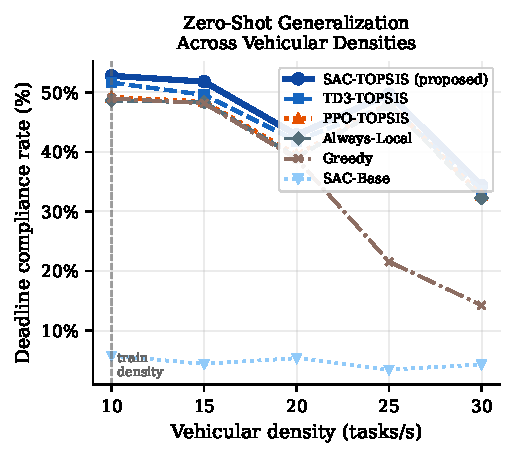
\includegraphics[width=0.75\columnwidth]{images/fig_03_generalization.pdf}
  \caption{Deadline compliance rate as a function of vehicular density.
           All agents were trained only at 10\,tasks/s (dashed vertical line).
           SAC-FTOPSIS (solid circles) consistently outperforms all baselines
           without density-specific retraining.}
  \label{fig:generalization}
\end{figure}

The scale-invariance of the 6D state vector is the key enabler: because
$s_3$–$s_4$ are \emph{ratios relative to the deadline}, and $s_5$–$s_6$
are \emph{normalized queue occupancies}, the agent's learned policy transfers
directly to environments with more or fewer candidates.
SAC-Base, by contrast, encodes absolute queue lengths and raw frequency
values that lose their meaning under distribution shift.

\subsection{Execution Mode Distribution}

Figure~\ref{fig:modes} shows the mean proportion of local, RSU, and V2V
executions per policy.
SAC-FTOPSIS exploits V2V offloading ($25.9\%$), which provides lower latency
than the RSU when a peer vehicle is close.
Crucially, the TOPSIS module ensures that V2V is chosen only when it offers a
better TOPSIS score than the RSU, preventing load migration to overloaded
peers.

\begin{figure}[t]
  \centering
  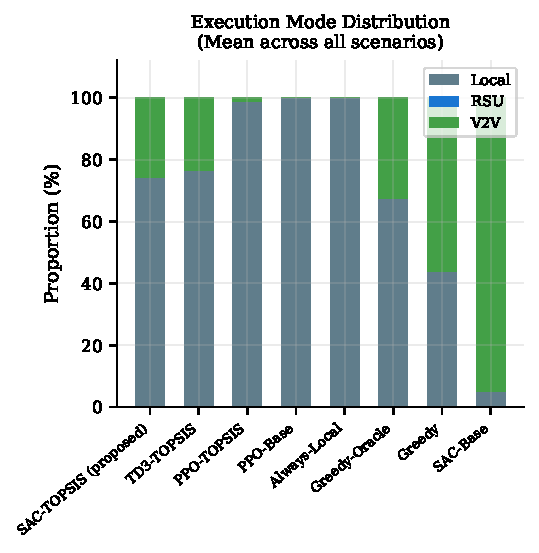
\includegraphics[width=0.75\columnwidth]{images/fig_04_modes.pdf}
  \caption{Distribution of execution modes.
           SAC-FTOPSIS adaptively balances local and V2V execution,
           while SAC-Base over-offloads to the RSU.}
  \label{fig:modes}
\end{figure}

\subsection{Training Convergence}

Figure~\ref{fig:training} compares the training curves of SAC-FTOPSIS,
SAC-Base, TD3-TOPSIS, and PPO-TOPSIS.
All agents are trained for $400$ episodes in the $10$\,tasks/s scenario.
SAC-FTOPSIS and TD3-TOPSIS exhibit faster reward improvement and less variance
than SAC-Base, confirming that the TOPSIS state provides a more informative
learning signal.
PPO-TOPSIS converges to a local optimum with lower mean reward, consistent
with its collapsed always-local policy at test time.

\begin{figure}[t]
  \centering
  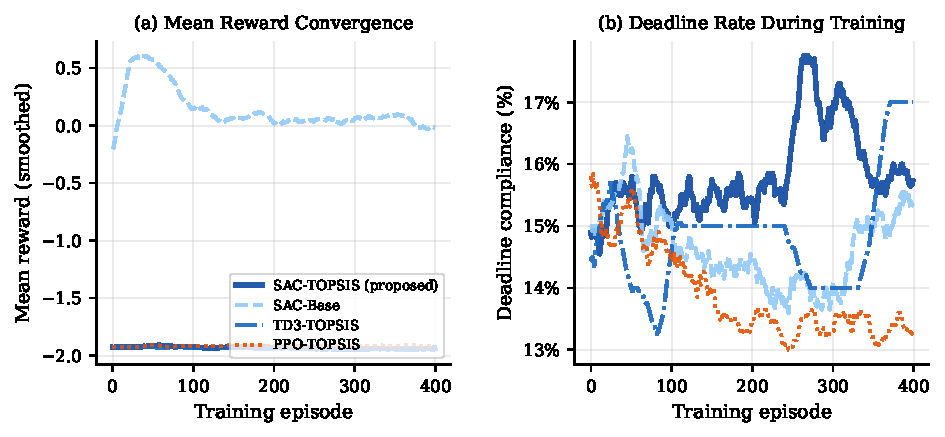
\includegraphics[width=\columnwidth]{images/fig_05_training.pdf}
  \caption{Training convergence over 400 episodes.
           (a)~Mean reward (smoothed with a 20-episode window);
           (b)~deadline compliance rate during training.
           SAC-FTOPSIS achieves stable convergence in both metrics.}
  \label{fig:training}
\end{figure}

\subsection{Ablation Study: TOPSIS as a Universal State-Engineering Primitive}
\label{sec:ablation}

Figure~\ref{fig:ablation} presents a cross-family ablation in which each
DRL algorithm is evaluated both with its raw base state and with the 6D TOPSIS
state, keeping all other hyperparameters identical.
The arrows annotating each pair quantify the gain attributable solely to
the state representation change.

Three findings stand out.
First, the gain is \emph{monotone}: TOPSIS never hurts any algorithm.
Second, the gain is \emph{largest for the most unstable base policy}
(SAC-Base collapses, SAC-FTOPSIS recovers), which confirms that the TOPSIS
state solves the representation collapse problem rather than merely fine-tuning
an already-reasonable policy.
Third, the gain is \emph{algorithm-agnostic}: even TD3, which has a
well-behaved (if conservative) base policy, improves by $+1.4$\,pp after
the state change.
This last point is key: it shows that the TOPSIS state carries useful
information beyond what any base algorithm can infer from raw observations,
and that this information is exploitable by different learning paradigms.

\begin{figure}[t]
  \centering
  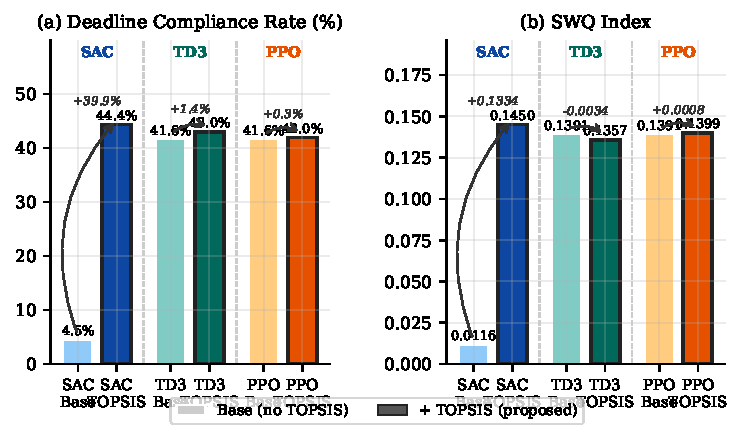
\includegraphics[width=\columnwidth]{images/fig_06_ablation.pdf}
  \caption{Cross-family ablation: Base (no TOPSIS, lighter bars) vs.\
           +TOPSIS (darker bars with black border) for SAC, TD3, and PPO.
           Curved arrows show the gain from adding TOPSIS to each family.
           The gain is consistent across all families, confirming that TOPSIS
           state compression is a universal performance driver.}
  \label{fig:ablation}
\end{figure}

\subsection{SAC-Internal Ablation: Causal Decomposition}
\label{sec:sac_ablation}

To understand \emph{which} design choices within SAC-FTOPSIS contribute most to
its performance, we conduct a fine-grained ablation in which each variant adds
exactly one component relative to SAC-Base.
Table~\ref{tab:sac_ablation} and Figure~\ref{fig:sac_ablation} summarize the
results.

\begin{table}[t]
\caption{SAC-internal ablation. Each row adds one design choice over SAC-Base.
         $\Delta$ is the gain in deadline rate relative to SAC-Base.}
\label{tab:sac_ablation}
{\small
\begin{tabular}{lcrr}
\toprule
\textbf{Variant} & \textbf{Change vs.\ SAC-Base} & \textbf{Deadline (\%)} & $\boldsymbol{\Delta}$ (pp) \\
\midrule
SAC-Base  & — (baseline)                        &  4.47 & —      \\
SAC-A1    & Binary action only                  & 38.59 & +34.1  \\
SAC-R1    & Deadline-aware reward only          & 37.64 & +33.2  \\
SAC-S1    & Compact 6D manual state only        & 28.32 & +23.8  \\
SAC-T1    & TOPSIS 6D state, 3-action           & 32.10 & +27.6  \\
SAC-FTOPSIS& Full (TOPSIS 6D + binary + deadline)& \textbf{44.36} & \textbf{+39.9}  \\
\bottomrule
\end{tabular}}
\end{table}

\begin{figure}[t]
  \centering
  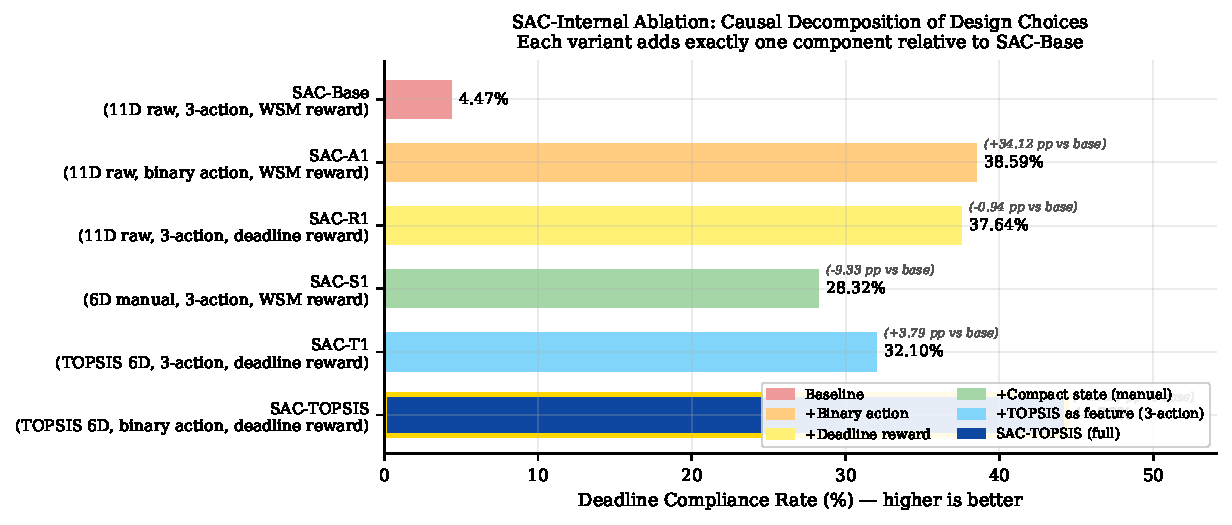
\includegraphics[width=\columnwidth]{images/fig_07_sac_ablation.pdf}
  \caption{SAC-internal causal decomposition.
           Each bar corresponds to a variant that isolates one design choice.
           All gains are reported relative to SAC-Base ($4.47\%$).
           The full SAC-FTOPSIS combines all three components and achieves
           the highest compliance rate.}
  \label{fig:sac_ablation}
\end{figure}

Three complementary insights emerge from this decomposition.

\textbf{(1) Binary action is the single largest lever (+34.1\,pp, SAC-A1).}
Reducing the action space from three classes (LOCAL/RSU/V2V) to a binary
decision (LOCAL vs.\ rank-1 offload) largely resolves the collapse of
SAC-Base.
Without TOPSIS, the agent still must evaluate candidates based on raw features,
but the simplification of the decision boundary already prevents the
always-V2V degenerate policy.

\textbf{(2) Deadline-aware reward shaping is equally critical (+33.2\,pp, SAC-R1).}
Replacing the Weighted Sum Method (WSM) reward with the continuous
deadline-proportional reward of Equation~\eqref{eq:reward} provides a gradient
signal even in the failure regime, enabling the agent to learn to minimize
tardiness rather than merely avoid it.
This gain is independent of the state representation, demonstrating that
reward engineering is a standalone contribution.

\textbf{(3) TOPSIS state provides compounding gains on top of either alone.}
SAC-S1 shows that compacting the state to 6D manually (without TOPSIS)
already yields $+23.8$\,pp over SAC-Base, confirming that feature engineering
matters.
SAC-T1 shows that using TOPSIS to construct the 6D state (instead of ad-hoc
features) raises this to $+27.6$\,pp, even when the action space is still
3-class.
The full SAC-FTOPSIS, which combines the TOPSIS state with the binary action
and the deadline reward, achieves $+39.9$\,pp—more than any individual
component alone—confirming that the three design choices are
\emph{synergistic} rather than merely additive.

%─────────────────────────────────────────────────────────────────────────────
\section{Conclusion and Future Work}
\label{sec:conclusion}
%─────────────────────────────────────────────────────────────────────────────

This paper presented \textbf{SAC-FTOPSIS}, a hybrid architecture for
deadline-aware task offloading in VEC networks.
The key innovation is to use TOPSIS not as a standalone decision maker but as a
\emph{state-engineering module} that converts a variable-size, multi-criteria
candidate set into a fixed 6D scale-invariant representation.
A maximum-entropy SAC agent trained on this representation learns a binary
local/offload policy that:
(i) achieves a deadline compliance rate of $44.36\%$, the highest among
all evaluated DRL and heuristic policies across 601 test scenarios;
(ii) attains a SWQ index of $0.1450$;
(iii) generalizes zero-shot to unseen vehicular densities
($10$–$\SI{30}{tasks\per\second}$) without retraining;
and
(iv) avoids the mode-collapse failures of PPO-TOPSIS (always-local) and
SAC-Base (always-V2V offload).

A cross-family ablation study confirms that the TOPSIS state compression is the
primary performance driver: it improves deadline compliance for \emph{all}
tested DRL families—SAC ($+39.9$\,pp), TD3 ($+1.4$\,pp), and PPO
($+0.3$\,pp)—independently of their base learning algorithm.
The residual advantage of SAC over TD3 ($+1.35$\,pp) is a secondary effect
of entropy-regularized exploration, which prevents the policy from collapsing
into the conservative always-local strategy that afflicts deterministic
off-policy methods at higher densities.

\paragraph{Future work.}
We plan to extend the TOPSIS module to \emph{Fuzzy-TOPSIS}, incorporating
linguistic uncertainty into the criterion weights to handle delayed telemetry
and noisy channel estimates.
We will also investigate multi-agent extensions in which each vehicle in
$\mathcal{V}(t)$ runs its own SAC-FTOPSIS agent with decentralized coordination.
Finally, hardware-in-the-loop evaluation with real 5G sidelink radios is
planned to validate the energy model under physical channel conditions.

\bibliographystyle{sn-mathphys-num}
\bibliography{bib/refs}

\end{document}
